%!TEX root = main.tex

\chapter{Introduction}
\label{introduction}

\begin{figure}[h!]
	\centering
	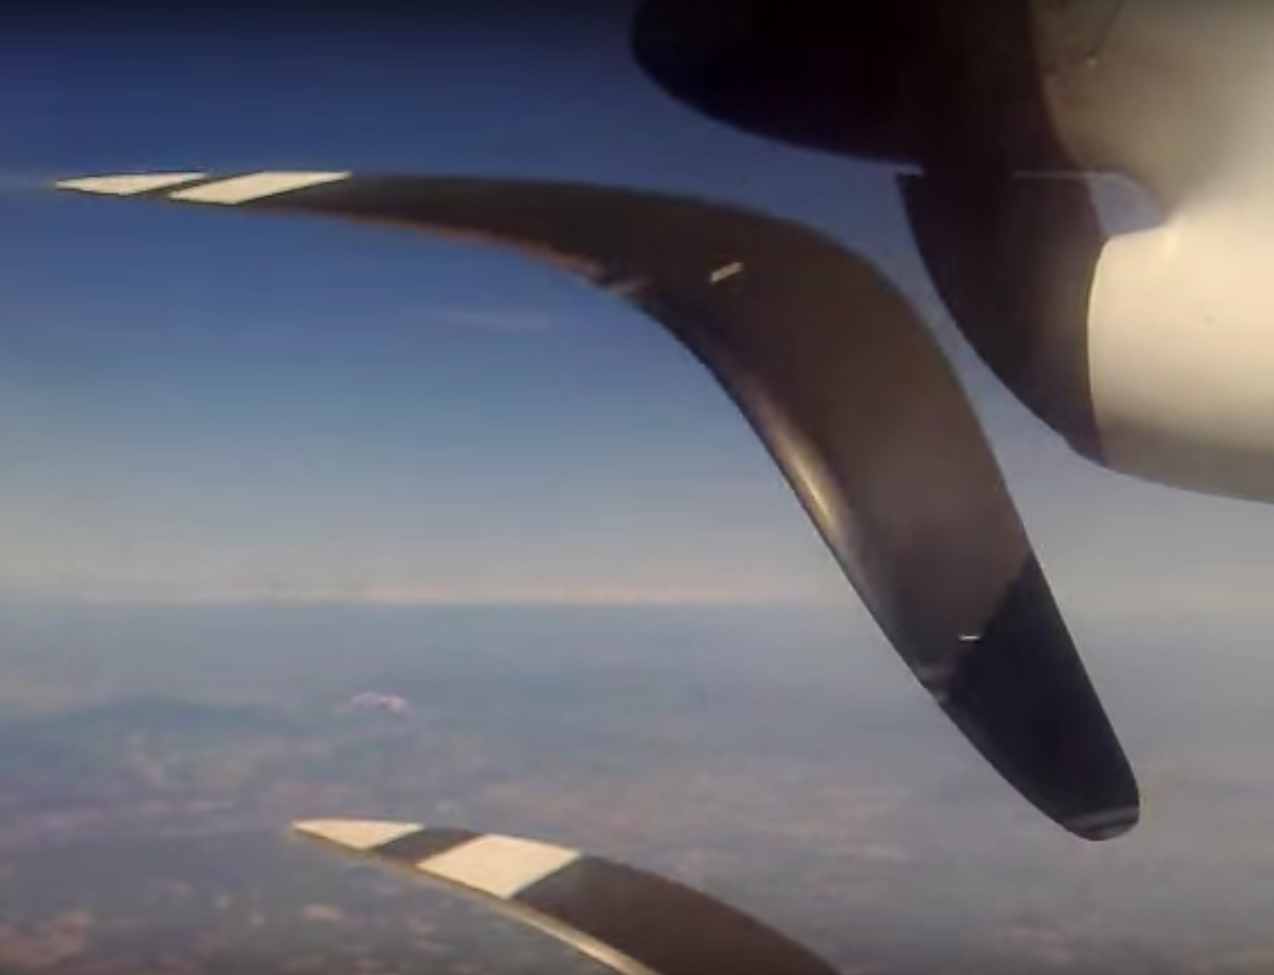
\includegraphics[width=\textwidth]{intro}
	\caption[shortCaption]
	{Weird effects of digital signals in video}
	\label{fig:label}
\end{figure}
\clearpage

This section tries to make sure we are all on the same page. It goes through some mathematics notation and principles of digital audio.\\
If you rather want a video format revision of digital audio (I mean, it's \the\year, of course you want), I can recommend \href{https://www.youtube.com/watch?v=cIQ9IXSUzuM}{D/A and A/D | Digital Show and Tell (Monty Montgomery @ xiph.org) }\footnote{https://www.youtube.com/watch?v=cIQ9IXSUzuM}. Some of the points in the video go beyond what we are doing here and vice versa, so don't purely rely on the video though. \\
Ideally, if you throughly understood the introduction section, you should be able to go through the remaining chapters with tempo.\\

\section{About this document}
Please report any mistakes, errors etc to \href{mailto:ptrk.lechner@gmail.com}{ptrk.lechner@gmail.com}.\\

Some information in this document is relevant for understanding its contents but not relevant for the exam. For example in chapter \ref{Modulation} we will find a really complicated result of an equation. The point there is just that it's complicated. And it is shown how complicated, but this is nothing to be learned by heart. Importance is tried to be made clear using the following formats:\\

\bgInfo{
Text, figures, and equations with a gray background like this are background information that is not to be learned by heart.}

\video{
This document tries to explain digital signals. It does this by use of audio signals mainly. Sometimes video analogies are given. These are also not relevant for the exam.
}

\important{Very important things are framed.}

pd objects will always be in courier new and square brackets. Like this: \pd{metro}



\section{About plotting signals}

We will need to plot a lot of signals in order to understand them better. Most of the time, such a plot will look like figure \ref{fig:simpeSine}.

\begin{figure}[h!]
	\centering
	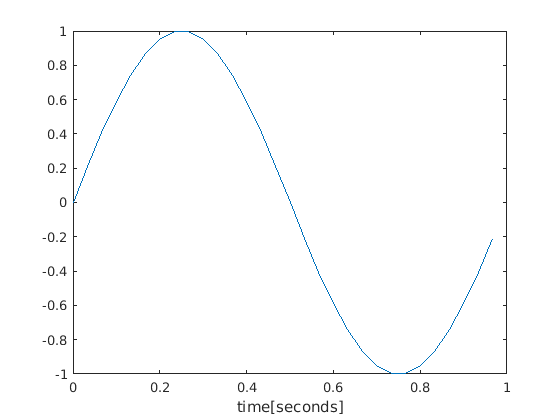
\includegraphics[width=11cm]{simpleSine}
	\caption[simple sine plot]
	{Sine wave, 1Hz, sampled at 30Hz sample rate}
	\label{fig:simpeSine}
\end{figure}

This plot looks nice but it has a problem. The sine wave is sampled at a sampling rate of 30 Hz, but we see a continuous line. This ``connection of the dots'' is created by plotting. It is kind of similar to what our \textit{digital-to-analog-converter} does. It somehow\footnote{linear interpolation in case of the plot} interpolates the values we have. \\
This can be misleading, so we should actually plot something more like figure \ref{fig:scatter}. Often we can see plots that look like figure \ref{fig:stem} as well when a signal is analyzed.

\begin{figure}[H]
	\centering
	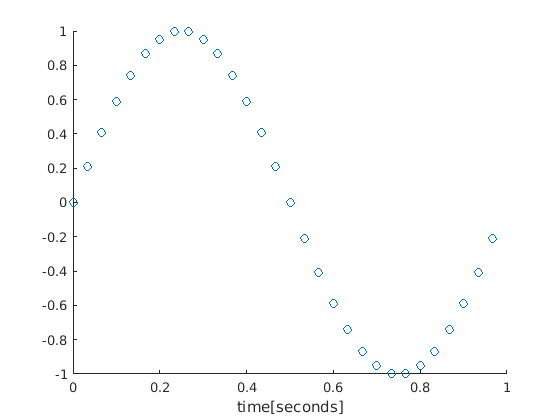
\includegraphics[width=11cm]{sineScatter}
	\caption[shortCaption]
	{Sine wave, 1Hz, sample rate 30Hz, scatter-plot}
	\label{fig:scatter}
\end{figure}



\begin{figure}[H]
	\centering
	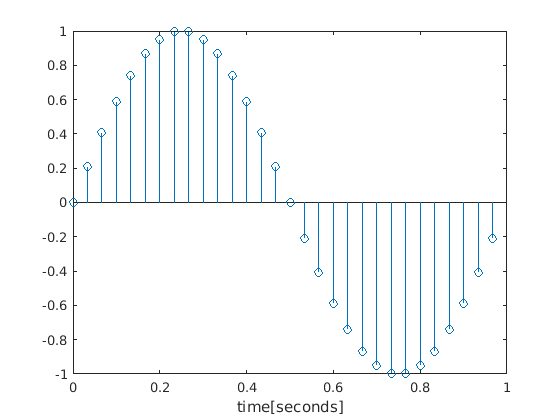
\includegraphics[width=11cm]{sineStem}
	\caption[shortCaption]
	{Sine wave, 1Hz, sample rate 30Hz, stem-plot}
	\label{fig:stem}
\end{figure}


So why don't we always do a stem- or scatter-plot? Simply because it gets too crowded with our usual sampling rates in audio. It just works with very low sampling rates or very short signals.\\
\begin{figure}[H]
	\centering
	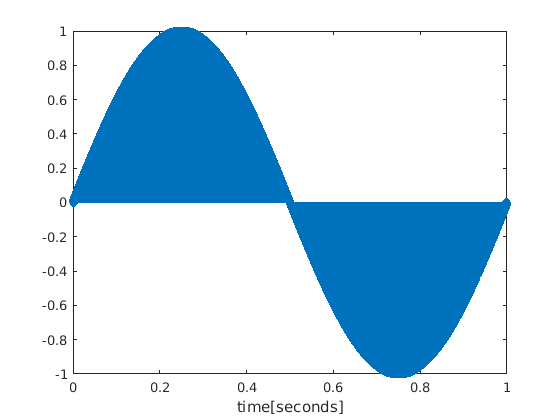
\includegraphics[width=11cm]{stem44100}
	\caption[shortCaption]
	{Sine wave, 1Hz, sample rate 44100Hz, stem-plot}
	\label{fig:label}
\end{figure}
\textbf{But we should never forget that we don't actually have the values in between the dots. Digital signals are not defined between their sampled points.}

\section{What is aliasing?}
Aliasing in audio means problems caused by signals that exceed the nyquist rate.\\
The nyquist rate,let's call it $f_n$ for now, is defined by the half of the sample rate ($f_s$). So,
\begin{equation}
	f_n=\frac{f_s}{2}
\end{equation}
A digital system can only describe signals up to his nyquist rate. If we try to make signals higher than this frequency, we will fail and encounter strange effects.\\
Visually speaking, frequencies higher than nyquist fold back. So, let's assume we have a sampling rate of 100Hz. Nyquist would be at 50Hz. If we try to synthesize a sine wave with 51Hz, what we will get is a 49Hz one. If we try to make a 52Hz one, we will get 48Hz. So you see, it simply folds back.

\begin{framed}
	\textbf{Video analogies}\\
	Aliasing in graphics usually means \textit{spacial} aliasing, so aliasing in the space domain. This is what we see in figure \ref{fig:spAlias}. But there is also time domain aliasing in film. It is actually more natural to think about the sampling rate in audio as the same as the frame rate in video. For some really weird effects that arise in video due to time domain aliasing see \href{https://www.youtube.com/watch?v=LVwmtwZLG88}{airplane}\footnotemark , \href{https://www.youtube.com/watch?v=GBtHeR-hY9Y}{Water experiment}\footnotemark or \href{https://www.youtube.com/watch?v=jcOKTTnOIV8}{Guitar strings}\footnotemark .
	\begin{center}
		% \centering
		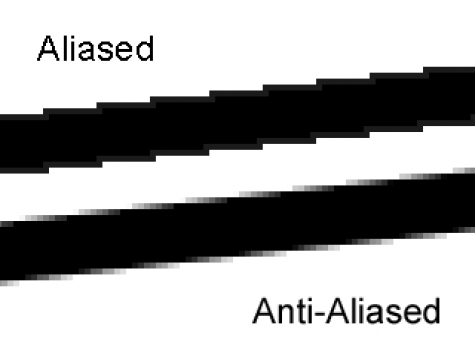
\includegraphics[width=7cm]{spacialAliasing1.png}
		\captionof{figure}{Spacial aliasing in graphics. The ``frequency'' of the intended pixels is to high for the actual pixels.}
		\label{fig:spAlias}
	\end{center}
	The particularly strange effects in the airplane example above are caused by the rolling shutter of a CMOS sensor. Since it is not sampling the incoming light uniformly (at the same time) the image is distorted.
\end{framed}
\footnotetext[2]{https://www.youtube.com/watch?v=LVwmtwZLG88}
\footnotetext[3]{https://www.youtube.com/watch?v=GBtHeR-hY9Y}
\footnotetext[4]{https://www.youtube.com/watch?v=jcOKTTnOIV8}


In figure \ref{fig:cosAlias} you can see a visualization of aliasing in the time domain.

\begin{figure}[H]
	\centering
	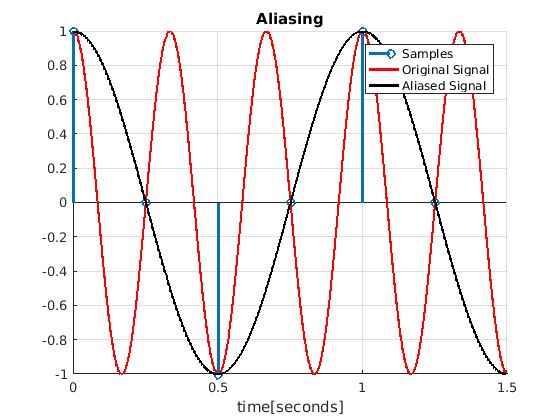
\includegraphics[width=\textwidth]{aliasingSine}
	\caption[shortCaption]
	{Aliasing visualized in the time domain. A sampling rate of 4 Hz is used. Therefore frequencies will fold above 2 Hz, which is the nyquist frequency. The input cosine has a frequency of 3 Hz, labeled ``Orginal Signal''. What we would get is the sampled points. If these are digital-to-analog converted, we would get what is labeled ``Aliased signal '' in this plot, so a 1 Hz cosine.}
	\label{fig:cosAlias}
\end{figure}



\begin{figure}[H]
	\begin{center}
		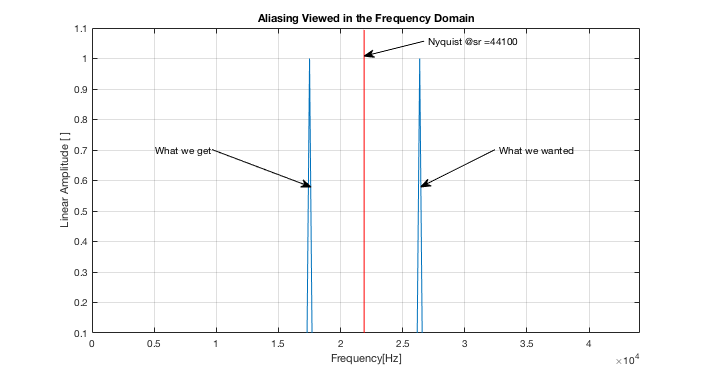
\includegraphics[width = \textwidth]{aliasingFreqDomain.png}
		\caption[Aliasing in the Frequency Domain]
		{Here we can see the phenomenon of aliasing in the frequency domain. We try to synthesize a sine wave at about 26kHz. At a sampling rate of 44100 Hz, this is not possible, nyquist is at 22050 Hz. What we actually get is a sine wave at about 17kHz. In this plot, the nyquist frequency is marked with the red line. Please note that the distance between the red line to both peaks is identical. This is why the phenomeno is also called \textit{fold-back}}
		\label{fig:name}
	\end{center}
\end{figure}





\section{Scaling and Mapping Signals}
It is an important skill to be able to scale signals from one range to another. We need it a lot and we will be able to think about signals more easily if we mastered this task. It's actually quite simple, we just have to imagine the signals visually.\\
So what exactly do we have to do here? We are confronted with the following problem: Given some signal, say, a sine wave with its maximum at the value 1 and its minimum at the value -1. How to bring it to a different range, say, 0-10?\\
It helps me a lot to solve this problem in two parts: first get the input in the range 0-1, then from there go to the desired range. What can we do to the signal? Let's take a sine wave:

\begin{figure}[h!]
	\centering
	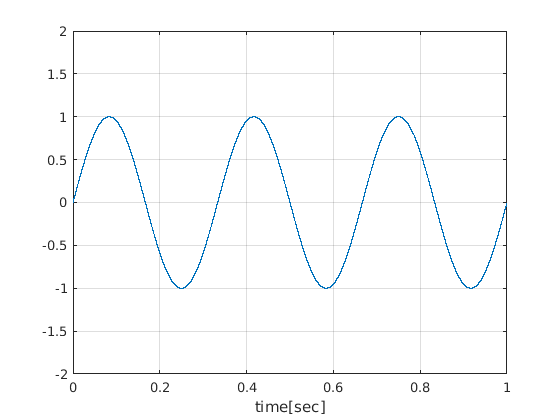
\includegraphics[width=11cm]{stdSine.png}
	\caption[a sine wave]
	{a sine wave}
	\label{fig:aSine}
\end{figure}
Well we can add and subtract to move the wave vertically, so let's add 1 to move it up:

\begin{figure}[h!]
	\centering
	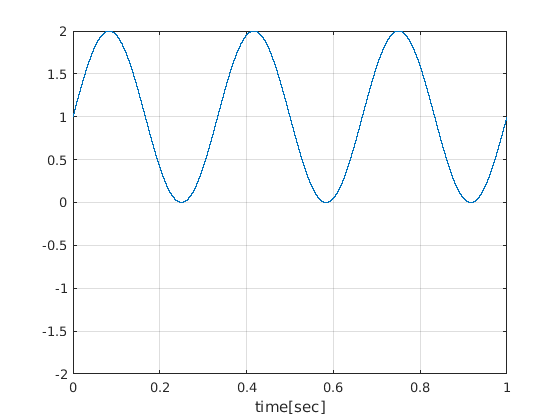
\includegraphics[width=11cm]{sinePlusOne.png}
	\caption[a sine wave]
	{the same sine wave, 1 added to a each sample, therefore shifted upwards.}
	\label{fig:aShiftedSine}
\end{figure}

So we can move signals around by adding constant values. We can scale them by multiplication. So if we take our sine that now ranges from 0 to 2 and multiply it by 0.5, we get whats in figure \ref{fig:sine01}.

\begin{figure}[h!]
 	\centering
 	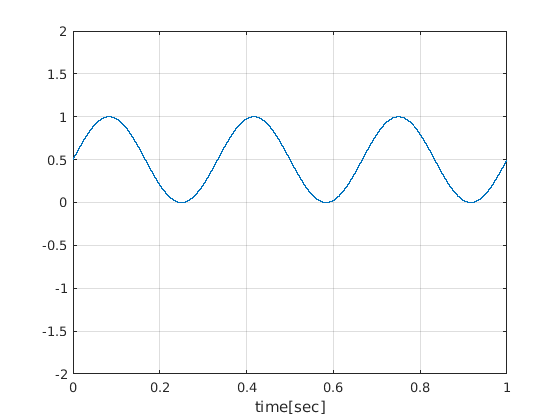
\includegraphics[width=11cm]{sine01.png}
 	\caption[sine 0 to 1]
 	{Sine with a range of 0-1. Obtained by taking a sine wave, adding 1 and dividing by two afterwards.}
 	\label{fig:sine01}
 \end{figure}

Using what we got now in figure \ref{fig:sine01}, we can just multiply by 10, easy! Beware that there are always multiple solutions to this kind of a problem. Try to find another one for the problem above!

\begin{question}
Let's take a sine wave that has it's minimum at 2 and it's maximum at 5. What do we have to do to get it into a -1 to 1 range?
\end{question}
\begin{Answer}
We could subtract 3.5 to center the wave around zero first. Afterwards we take care of the amplitude by multiplying by $\frac{2}{3}$ (since the initial wave has a peak-to-peak amplitude of three and we want a peak-to-peak amplitude of 2)
\end{Answer}



\section{What's DC-Offset?}

What we did above by adding a constant value to a signal can be called adding DC-offset (``Gleichspannungsversatz''), DC-Bias or a DC component. These are different words for the same thing.\\
DC-offset can also be encountered in signals we recorded (caused by old or broken equipment mainly). But we have seen that we can also generate DC-offset.\\
To state it again clearly:
\begin{framed}
DC-Offset is a constant value over time, or a constant offset from the zero value in Y. So for example in figure \ref{fig:sine01} we see a DC-offset of 0.5 since subtracting this value would center the wave around 0.
\end{framed}
If we try to think how this kind of signal looks in the frequency domain we find that it is energy at 0Hz. In figure \ref{fig:dcViz} you can see a couple of cosine waves plotted. This should hep imagine that a constant signal, a signal that does not move a all, can be described by a cosine with 0 Hz and a certain amplitude.

\begin{figure}[h!]
	\centering
	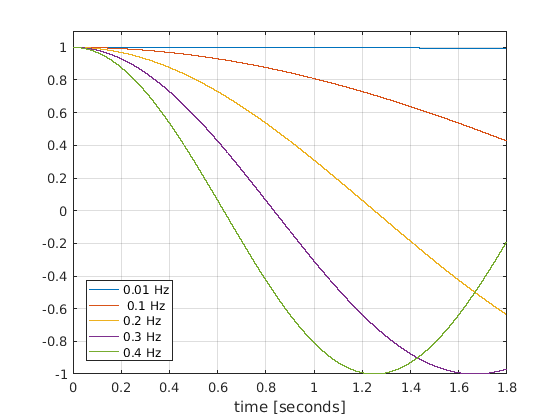
\includegraphics[width=11cm]{dcOffsetViz}
	\caption[shortCaption]
	{Cosines with different very low frequencies approaching 0Hz, so DC offset.}
	\label{fig:dcViz}
\end{figure}

Let's quickly state this differently, so we can appreciate the surprising connections between DC-offset and an impulse. A DC-offset signal is a signal consisting of constant values, so for example $\{...,1,1,1,1,1,1,...\}$. Its spectrum is a single peak at 0Hz, so the spectrum's values look like $\{..., 0,0,0,1,0,0,0,...\}$\footnote{Why is the $1$, so the 0 Hz component not at the beginning of the list? Or is it not 0 Hz? The 1 is supposed to be at 0Hz, and it is centered in this list because doing an FFT actually always gets us a two-sided spectrum. You can ignore this fact until the FFT chapter, and pretend that the list starts with 1 (which wouldn't be wrong also). }


\begin{figure}[H]
	\begin{center}
		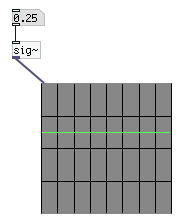
\includegraphics[width = 5cm]{dcPd.png}
		\caption[Dc-offset in pd]
		{One of the ways to generate a DC signal in pd.}
		\label{fig:name}
	\end{center}
\end{figure}




% \comm{explanations and visualizations missing}

\section{What's an Impulse?}

Impulses are very useful signals. We can produce an impulse using the \pd{dirac\textasciitilde} object.

\begin{figure}[H]
	\begin{center}
		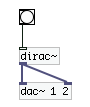
\includegraphics[width = 3cm]{dirac.png}
		\caption[The dirac object]
		{The \pd{dirac\textasciitilde} object produces an impulse if we send it a \texttt{bang}.}
		\label{fig:name}
	\end{center}
\end{figure}
\bgInfo{
Different people will define what's an impulse in different ways:
\begin{itemize}
	\item A sound engineer might tell you, that clapping your hands or shooting with a gun creates an impulse
	\item a mathematician will maybe give you the definition of the \textit{dirac delta function} (that's where the name for pd's impulse object comes from)
	\item Somebody working with discrete (so digital) signals will give you rather the definition of the Kroneker delta function.
\end{itemize}


}

For us, strictly speaking, an impulse will be a signal that contains only zeros, but one sample with the value one. We can see such an impulse in figure \ref{fig:unitImpulse}. On the x-axis, we have the time in samples\footnote{Don't be irritated by the fact that the sample numbers on the x-axis are ranging from $-5$ to $5$. You can just as well imagine them going from 0 to 10 or 1 to 11. It doesn't really matter. However, this way of displaying an impulse is very common since if the impulse is filtered, it's symmetry is an important factor.}.


\begin{figure}[H]
	\begin{center}
		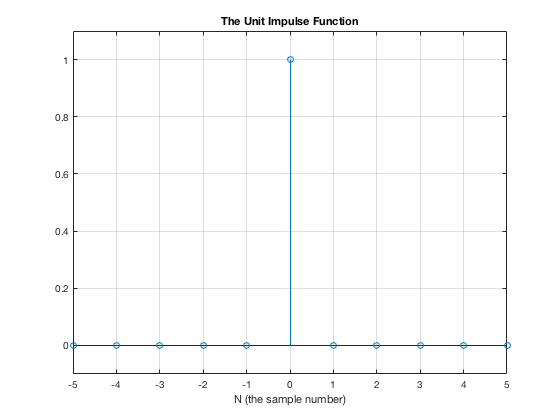
\includegraphics[width = \textwidth]{unitImpulse.png}
		\caption{caption}
		\label{fig:unitImpulse}
	\end{center}
\end{figure}

So in the time domain, an impulse's samples have the values $\{...,0,0,0,1,0,0,0,...\}$. If we look at it's spectrum, we will find that it contains all frequencies, there is just a flat line in the spectrum (you can see an impulse's spectrum in figure \ref{fig:impToDc} also.). The spectrum has a \textit{constant value}, something like $\{..,1,1,1,1,1,1,...\}$. Do these two lists look familiar? Right, it is exactly the opposite of the DC-offset signal.



\section{How to describe audio mathematically}

If we want to talk about signals, or if we want to analyze them, it is often useful to look at the problem mathematically. First, let's introduce some conventions. They might look unfamiliar or complicated. But in fact it is not very complicated and knowing these conventions makes it easy to communicate (e.g. reading scientific papers about our topics or explaining something to another person).

\subsection{signals}

Usually we describe a \textit{digital} signal by a name, say $x$, (but you can call it however you want). If we want to talk about the individual samples, or values of the (mono) signal, we can use a subscript or parenthesis. So if the fifth sample of $x$ is 1, we could write:

\begin{equation}
	x_5=1
\end{equation}
or
\begin{equation}
	x(5)=1
\end{equation}
Oftentimes we like to talk about a signal more generally and we use $n$ as a place holder for this index, so we might write $x_n$, meaning the nth sample of $x$.

\subsubsection{sine waves}
We use sine waves a lot. The syntax can get a bit overwhelming at first, so let's quickly explain what's going on in a standard sine wave oscillator.
\begin{equation}
	x(t) = A \cdot sin(2\pi f t + \phi)
\end{equation}
Where $f$ is the frequency in Hertz and $t$ is the time in seconds. $\phi$ Is a (possibly constant) phase offset and $A$ can be used to scale the whole thing. Since cosine and sine have their peaks at -1 and 1, $A$ will be the amplitude. If $A$ is set to 0.5, the resulting signal will have it's peaks at -0.5 and 0.5. \\
The upper equation is rather complete. Most of the time, we will just ignor the phase and the amplitude and just write:
\begin{equation}
	x(t) = sin(2\pi f t )
\end{equation}

Sometimes, we will simplify even more and just write $sin(a)$ or $sin(b)$ or similar.\\
\begin{mdframed}[backgroundcolor=black!10,rightline=false,leftline=false]
In literature, we sometimes encounter $x(t) = sin(t \cdot \omega)$. $\omega$ stands for a ``frequency''(actually for the rotational speed) in \textit{radians per second}. $2\pi$ radians per second are 1 Hz and we can therefore convert radians per second to frequency, $v$, with:
\begin{equation}
  	v = \omega / 2\pi
  \end{equation}
This notation is only covered since it is very common, but it will not be used here, since it is considered more intuitive to work with frequency in Hz.
\vspace{0.5cm}

\textbf{What is actually the significance of using either $sin$ or $cos$?}\\
In most cases for us, this does not matter at all. The difference between sine and cosine is just in phase. Since we are most of the time describing a sine (or cosine) wave oscillator as a function of time, the only difference between the two would be their phase if given some moment in time. This is nothing one could hear also.

\end{mdframed}
% \comm{work in progress.}

\subsection{systems}
There are many ways to describe systems. Digital LTI systems (Linear, time invariant Systems) can be described using
\begin{itemize}
	\item difference equations
	\item Block diagrams
	\item Transfer Functions
	\item and other things.
\end{itemize}

For us, the most important ways to describe a system are block diagrams and difference equations.

\subsection{systems}

There are multiple ways in which we can describe linear time invariant (LTI) systems. We will talk more about this in chapter \ref{chap:filters}. Here, we will just look at how \textit{difference equations} work. These are one possibility to describe a digital LTI system. They are the discrete equivalent of difference equations. It's really not that complicated:
\begin{equation}
	y(n) = x(n)
\end{equation}
Would be an equation that describes a system that does nothing. it takes the input sample, $x(n)$ does nothing and defines the output sample $y(n)$ with it.
Another really simple system would multiply its input by two:
\begin{equation}
	y(n) = x(n)\cdot 2
\end{equation}
It's getting interesting if we start playing with the index:
\begin{equation}
	y(n) = x(n-1)
\end{equation}
Is a delay by one sample.
\begin{equation}
	y(n) = x(n)+x(n-1)
\end{equation}
Takes it's input sample and the previous input sample, adds them together and spits it out. Can you imagine what this does? We'll get to it in chapter \ref{chap:filters}...

This is just a preview, but it really gets interesting if we start working with feedback:
\begin{equation}
 	y(n) = x(n)+y(n-1)
 \end{equation}


\section{Message Domain/Signal Domain}
This is not pure data specific although it might sound like it.
In pure data we can have audio signals. Audio signals are processed in buffers. They are just numbers, but these numbers are calculated at a rate of 44100 Hz \textit{all the time} if we choose to have our sample rate at 44100 Hz.\\
Messages on the other hand are not calculated that often and not all the time. Messages are processed \textit{on demand}. They are event based. This means that, for example, if we hit a note on our midi keyboard or enter a number in a \pd{Numberbox} this \textit{event} will pass through its following objects \textit{once}. Have a look at figure ~\ref{fig:mesSig} or at the patcher. Also note that pd helps us in understanding if we deal with message or signal domain:

\begin{itemize}
	\item pd is indicating the signal domain with thicker patch cords
	\item signal domain inlets/outlets are black (look closely)
	\item objects that deal with the signal domain have a tilde (\textasciitilde ) at the end of their name.
\end{itemize}
 % by indicating the signal domain with thicker patch cords and black inlets/outlets on the objects (look closely).

\begin{figure}[h!]
	\centering
	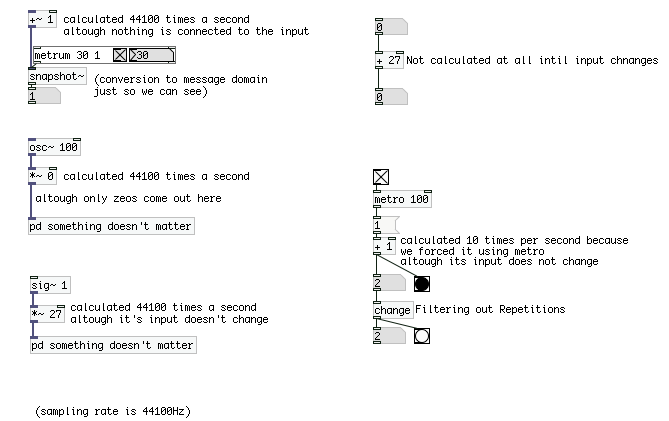
\includegraphics[width=\textwidth]{messageDomainSignalDomain}
	\caption[message domain vs. signal domain]
	{The patcher \texttt{messageDomainSignalDomain.pd} should demonstrate the differences between message domain and signal domain in pure data.}
	\label{fig:mesSig}
\end{figure}

\paragraph{How is this not specific to pure data?} The key points here are not specific to this programming language. If we, for example adjust the volume of a track in pro tools or ableton live or similar, then the information of our fader movement will also be in some kind of message domain.\\
One key aspect here is: some kind of conversion between the two is necessary if we want to switch between them. If we want to control the volume of an audio signal from the message domain we have a problem: we will get noisy output since the message domain is not running at sample rate. Look at a naive attempt to controlling the amplitude of a sine wave:

\begin{figure}[H]
	\centering
	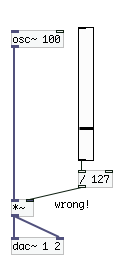
\includegraphics[width=5cm]{ampWrong}
	\caption[shortCaption]
	{The patcher \texttt{amplitudeWrongRight.pd} }
	\label{fig:label}
\end{figure}


And let's look at what kind of waveform it will produce:

\begin{figure}[H]
	\centering
	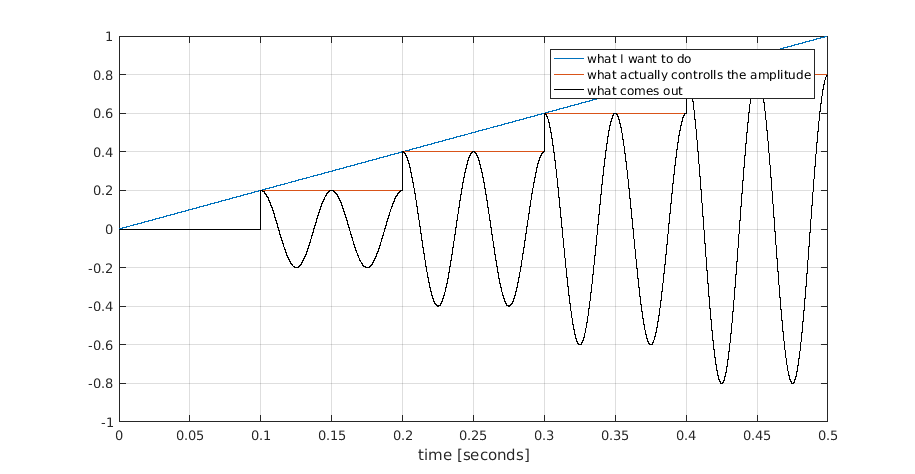
\includegraphics[width=\textwidth]{ampWrongViz}
	\caption[shortCaption]
	{This is a cosine wave at 20 Hz and the message domain running at 100 millisecond interval to make the effect more extreme and visible}
	\label{fig:label}
\end{figure}


This is a problem, since the sudden jumps produce clicks, crackling or zipper noise (reproduce or open the patcher and hear it for yourself!). These clicks are caused by the fact that the message domain just doesn't produce
the numbers at the rate of the sampling rate. It's too slow, so to speak.\\
In pure data (but also in general) this problem can be solved by interpolation. pure data offers the \pd{line\textasciitilde} object for this situation. It can be used to create signals at sampling rate and we can tell it to ramp to a specified value in a given amount of time. In figure \ref{fig:ampRight} we see it ramping to any value that comes from the \pd{/ 127} object within 20 milliseconds\footnote{20ms is just an example. It is a reasonable time for this kind of interpolation but really, it is just an example. It could just as well be 50 ms.}. This interpolation reduces the clicks and noise dramatically. Note that the output of \pd{line\textasciitilde} is in the signal domain (thick cable).

\begin{figure}[H]
	\centering
	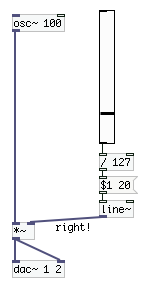
\includegraphics[width=4cm]{ampRight}
	\caption[shortCaption]
	{Controlling the amplitude of an oscillator. The interpolation done with \pd{line\textasciitilde} suppresses clicks. }
	\label{fig:ampRight}
\end{figure}


\section{Key Points}
\begin{itemize}
	\item Make sure you understand and know the mathematical notation. It will be how we talk in the remaining chapters.
	\item Make sure you understand what aliasing means in audio.
	\item Make sure you are comfortable with basic mathematical operations on signals, such as adding constants and multiplying with constants
	\item Make sure you understand the difference between message and signal domain and the problem with using a message domain ``signal'' controlling an audio stream.
	\item Make sure you know what the spectrum and time domain signal of an impulse and DC-Offset look like.
\end{itemize}
